\documentclass[12pt]{beamer}\usepackage[]{graphicx}\usepackage[]{color}
%% maxwidth is the original width if it is less than linewidth
%% otherwise use linewidth (to make sure the graphics do not exceed the margin)
\makeatletter
\def\maxwidth{ %
  \ifdim\Gin@nat@width>\linewidth
    \linewidth
  \else
    \Gin@nat@width
  \fi
}
\makeatother

\definecolor{fgcolor}{rgb}{0.345, 0.345, 0.345}
\newcommand{\hlnum}[1]{\textcolor[rgb]{0.686,0.059,0.569}{#1}}%
\newcommand{\hlstr}[1]{\textcolor[rgb]{0.192,0.494,0.8}{#1}}%
\newcommand{\hlcom}[1]{\textcolor[rgb]{0.678,0.584,0.686}{\textit{#1}}}%
\newcommand{\hlopt}[1]{\textcolor[rgb]{0,0,0}{#1}}%
\newcommand{\hlstd}[1]{\textcolor[rgb]{0.345,0.345,0.345}{#1}}%
\newcommand{\hlkwa}[1]{\textcolor[rgb]{0.161,0.373,0.58}{\textbf{#1}}}%
\newcommand{\hlkwb}[1]{\textcolor[rgb]{0.69,0.353,0.396}{#1}}%
\newcommand{\hlkwc}[1]{\textcolor[rgb]{0.333,0.667,0.333}{#1}}%
\newcommand{\hlkwd}[1]{\textcolor[rgb]{0.737,0.353,0.396}{\textbf{#1}}}%

\usepackage{framed}
\makeatletter
\newenvironment{kframe}{%
 \def\at@end@of@kframe{}%
 \ifinner\ifhmode%
  \def\at@end@of@kframe{\end{minipage}}%
  \begin{minipage}{\columnwidth}%
 \fi\fi%
 \def\FrameCommand##1{\hskip\@totalleftmargin \hskip-\fboxsep
 \colorbox{shadecolor}{##1}\hskip-\fboxsep
     % There is no \\@totalrightmargin, so:
     \hskip-\linewidth \hskip-\@totalleftmargin \hskip\columnwidth}%
 \MakeFramed {\advance\hsize-\width
   \@totalleftmargin\z@ \linewidth\hsize
   \@setminipage}}%
 {\par\unskip\endMakeFramed%
 \at@end@of@kframe}
\makeatother

\definecolor{shadecolor}{rgb}{.97, .97, .97}
\definecolor{messagecolor}{rgb}{0, 0, 0}
\definecolor{warningcolor}{rgb}{1, 0, 1}
\definecolor{errorcolor}{rgb}{1, 0, 0}
\newenvironment{knitrout}{}{} % an empty environment to be redefined in TeX

\usepackage{alltt}
\usepackage{graphicx}
\usepackage{tikz}
\setbeameroption{hide notes}
\setbeamertemplate{note page}[plain]
\usepackage{listings}

% get rid of junk
\usetheme{default}
\usefonttheme[onlymath]{serif}
\beamertemplatenavigationsymbolsempty
\hypersetup{pdfpagemode=UseNone} % don't show bookmarks on initial view

% named colors
\definecolor{offwhite}{RGB}{255,250,240}
\definecolor{gray}{RGB}{155,155,155}

\ifx\notescolors\undefined % slides

  \definecolor{foreground}{RGB}{80,80,80}
  \definecolor{background}{RGB}{255,255,255}
  \definecolor{title}{RGB}{255,199,0}
  \definecolor{subtitle}{RGB}{89,132,212}
  \definecolor{hilit}{RGB}{248,117,79}
  \definecolor{vhilit}{RGB}{255,111,207}
  \definecolor{lolit}{RGB}{200,200,200}
  \definecolor{lit}{RGB}{255,199,0}
  \definecolor{mdlit}{RGB}{89,132,212}
  \definecolor{link}{RGB}{248,117,79}

\else % notes
  \definecolor{background}{RGB}{255,255,255}
  \definecolor{foreground}{RGB}{24,24,24}
  \definecolor{title}{RGB}{27,94,134}
  \definecolor{subtitle}{RGB}{22,175,124}
  \definecolor{hilit}{RGB}{122,0,128}
  \definecolor{vhilit}{RGB}{255,0,128}
  \definecolor{lolit}{RGB}{95,95,95}
\fi
\definecolor{nhilit}{RGB}{128,0,128}  % hilit color in notes
\definecolor{nvhilit}{RGB}{255,0,128} % vhilit for notes

\newcommand{\hilit}{\color{hilit}}
\newcommand{\vhilit}{\color{vhilit}}
\newcommand{\nhilit}{\color{nhilit}}
\newcommand{\nvhilit}{\color{nvhilit}}
\newcommand{\lit}{\color{lit}}
\newcommand{\mdlit}{\color{mdlit}}
\newcommand{\lolit}{\color{lolit}}

% use those colors
\setbeamercolor{titlelike}{fg=title}
\setbeamercolor{subtitle}{fg=subtitle}
\setbeamercolor{frametitle}{fg=gray}
\setbeamercolor{structure}{fg=subtitle}
\setbeamercolor{institute}{fg=lolit}
\setbeamercolor{normal text}{fg=foreground,bg=background}
%\setbeamercolor{item}{fg=foreground} % color of bullets
%\setbeamercolor{subitem}{fg=hilit}
%\setbeamercolor{itemize/enumerate subbody}{fg=lolit}
\setbeamertemplate{itemize subitem}{{\textendash}}
\setbeamerfont{itemize/enumerate subbody}{size=\footnotesize}
\setbeamerfont{itemize/enumerate subitem}{size=\footnotesize}

% center title of slides
\setbeamertemplate{blocks}[rounded]
\setbeamertemplate{frametitle}[default][center]
% margins
\setbeamersize{text margin left=25pt,text margin right=25pt}

% page number
\setbeamertemplate{footline}{%
    \raisebox{5pt}{\makebox[\paperwidth]{\hfill\makebox[20pt]{\lolit
          \scriptsize\insertframenumber}}}\hspace*{5pt}}

% add a bit of space at the top of the notes page
\addtobeamertemplate{note page}{\setlength{\parskip}{12pt}}

% default link color
\hypersetup{colorlinks, urlcolor={link}}

\ifx\notescolors\undefined % slides
  % set up listing environment
  \lstset{language=bash,
          basicstyle=\ttfamily\scriptsize,
          frame=single,
          commentstyle=,
          backgroundcolor=\color{darkgray},
          showspaces=false,
          showstringspaces=false
          }
\else % notes
  \lstset{language=bash,
          basicstyle=\ttfamily\scriptsize,
          frame=single,
          commentstyle=,
          backgroundcolor=\color{offwhite},
          showspaces=false,
          showstringspaces=false
          }
\fi

% a few macros
\newcommand{\code}[1]{\texttt{#1}}
\newcommand{\hicode}[1]{{\hilit \texttt{#1}}}
\newcommand{\bb}[1]{\begin{block}{#1}}
\newcommand{\eb}{\end{block}}
\newcommand{\bi}{\begin{itemize}}
%\newcommand{\bbi}{\vspace{24pt} \begin{itemize} \itemsep8pt}
\newcommand{\bbi}{\vspace{4pt} \begin{itemize} \itemsep8pt}
\newcommand{\ei}{\end{itemize}}
\newcommand{\bv}{\begin{verbatim}}
\newcommand{\ev}{\end{verbatim}}
\newcommand{\ig}{\includegraphics}
\newcommand{\subt}[1]{{\footnotesize \color{subtitle} {#1}}}
\newcommand{\ttsm}{\tt \small}
\newcommand{\ttfn}{\tt \footnotesize}
\newcommand{\figh}[2]{\centerline{\includegraphics[height=#2\textheight]{#1}}}
\newcommand{\figw}[2]{\centerline{\includegraphics[width=#2\textwidth]{#1}}}



%------------------------------------------------
% end of header
%------------------------------------------------

\title{R package ggplot2}
\subtitle{STAT 133}
\author{\href{http://www.gastonsanchez.com}{Gaston Sanchez}}
\institute{Department of Statistics, UC{\textendash}Berkeley}
\date{\href{http://www.gastonsanchez.com}{\tt \scriptsize \color{foreground} gastonsanchez.com}
\\[-4pt]
\href{http://github.com/gastonstat/stat133}{\tt \scriptsize \color{foreground} github.com/gastonstat/stat133}
\\[-4pt]
{\scriptsize Course web: \href{http://www.gastonsanchez.com/stat133}{\tt gastonsanchez.com/stat133}}
}
\IfFileExists{upquote.sty}{\usepackage{upquote}}{}
\begin{document}


{
  \setbeamertemplate{footline}{} % no page number here
  \frame{
    \titlepage
  } 
}

%------------------------------------------------

\begin{frame}
\begin{center}
\Huge{\hilit{ggplot2}}
\end{center}
\end{frame}



%------------------------------------------------

\begin{frame}[fragile]
\frametitle{Scatterplot with \code{"ggplot2"}}

Terminology
\bi
  \item aesthetic mappings
  \item geometric objects
  \item statistical transformations
  \item scales
  \item non-data elements (themes \& elements)
  \item facets
\ei

\end{frame}

%------------------------------------------------

\begin{frame}[fragile]
\frametitle{Considerations}

Specifying graphical elements from 3 sources:
\bbi
  \item The data values (represented by the geometric objects)
  \item The scales and coordinate system (axes, legends)
  \item Plot annotations (background, title, grid lines)
\ei

\end{frame}

%------------------------------------------------

\begin{frame}[fragile]
\frametitle{Scatterplot with \code{geom\_point}}
\begin{knitrout}\scriptsize
\definecolor{shadecolor}{rgb}{0.969, 0.969, 0.969}\color{fgcolor}\begin{kframe}
\begin{alltt}
\hlkwd{ggplot}\hlstd{(}\hlkwc{data} \hlstd{= mtcars,} \hlkwd{aes}\hlstd{(}\hlkwc{x} \hlstd{= mpg,} \hlkwc{y} \hlstd{= hp))} \hlopt{+}
  \hlkwd{geom_point}\hlstd{()}
\end{alltt}
\end{kframe}

{\centering 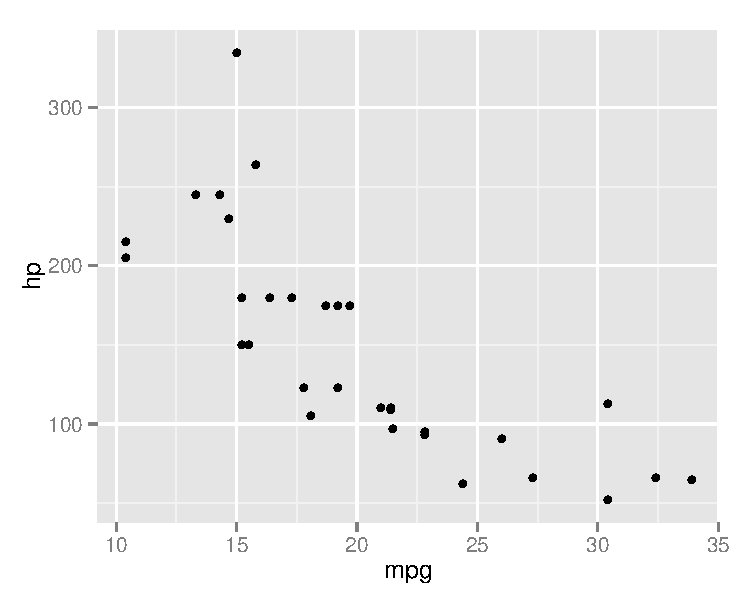
\includegraphics[width=.7\linewidth,height=.6\linewidth]{figure/unnamed-chunk-1-1} 

}



\end{knitrout}
\end{frame}

%------------------------------------------------

\begin{frame}[fragile]
\frametitle{Another \code{geom}}
\begin{knitrout}\scriptsize
\definecolor{shadecolor}{rgb}{0.969, 0.969, 0.969}\color{fgcolor}\begin{kframe}
\begin{alltt}
\hlkwd{ggplot}\hlstd{(}\hlkwc{data} \hlstd{= mtcars,} \hlkwd{aes}\hlstd{(}\hlkwc{x} \hlstd{= mpg,} \hlkwc{y} \hlstd{= hp))} \hlopt{+}
  \hlkwd{geom_line}\hlstd{()}
\end{alltt}
\end{kframe}

{\centering 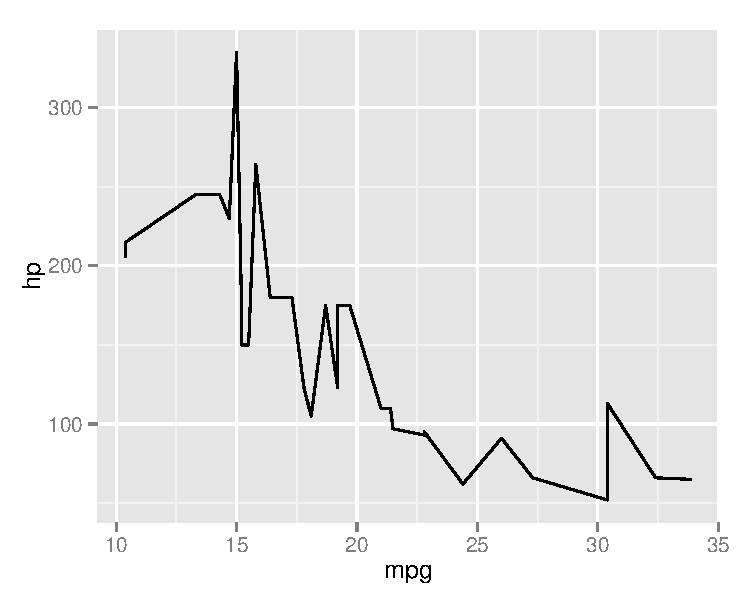
\includegraphics[width=.7\linewidth,height=.6\linewidth]{figure/unnamed-chunk-2-1} 

}



\end{knitrout}
\end{frame}

%------------------------------------------------

\begin{frame}
\begin{center}
\Huge{{\hilit Mapping Attributes \\ 
-vs- \\
Setting Attributes}}
\end{center}
\end{frame}

%------------------------------------------------

\begin{frame}[fragile]
\frametitle{Increase size of points}
\begin{knitrout}\scriptsize
\definecolor{shadecolor}{rgb}{0.969, 0.969, 0.969}\color{fgcolor}\begin{kframe}
\begin{alltt}
\hlkwd{ggplot}\hlstd{(}\hlkwc{data} \hlstd{= mtcars,} \hlkwd{aes}\hlstd{(}\hlkwc{x} \hlstd{= mpg,} \hlkwc{y} \hlstd{= hp))} \hlopt{+}
  \hlkwd{geom_point}\hlstd{(}\hlkwc{size} \hlstd{=} \hlnum{3}\hlstd{)}
\end{alltt}
\end{kframe}

{\centering 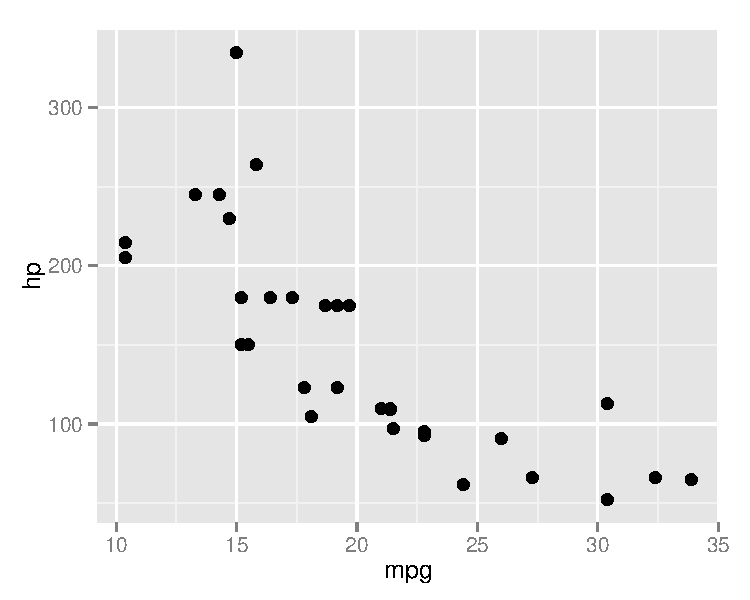
\includegraphics[width=.7\linewidth,height=.6\linewidth]{figure/xyplot_mtcars2-1} 

}



\end{knitrout}
\end{frame}

%------------------------------------------------

\begin{frame}[fragile]
\frametitle{How does it work?}
To increase the size of points, we \textbf{set} the aesthetic \code{size} to a constant value of 3 (inside the \textit{geoms} function):
\begin{knitrout}\footnotesize
\definecolor{shadecolor}{rgb}{0.969, 0.969, 0.969}\color{fgcolor}\begin{kframe}
\begin{alltt}
\hlopt{+} \hlkwd{geom_point}\hlstd{(}\hlkwc{size} \hlstd{=} \hlnum{3}\hlstd{)}
\end{alltt}
\end{kframe}
\end{knitrout}
\end{frame}

%------------------------------------------------

\begin{frame}[fragile]
\frametitle{Adding color}
\begin{knitrout}\scriptsize
\definecolor{shadecolor}{rgb}{0.969, 0.969, 0.969}\color{fgcolor}\begin{kframe}
\begin{alltt}
\hlkwd{ggplot}\hlstd{(}\hlkwc{data} \hlstd{= mtcars,} \hlkwd{aes}\hlstd{(}\hlkwc{x} \hlstd{= mpg,} \hlkwc{y} \hlstd{= hp))} \hlopt{+}
  \hlkwd{geom_point}\hlstd{(}\hlkwc{size} \hlstd{=} \hlnum{3}\hlstd{,} \hlkwc{color} \hlstd{=} \hlstr{"tomato"}\hlstd{)}
\end{alltt}
\end{kframe}

{\centering 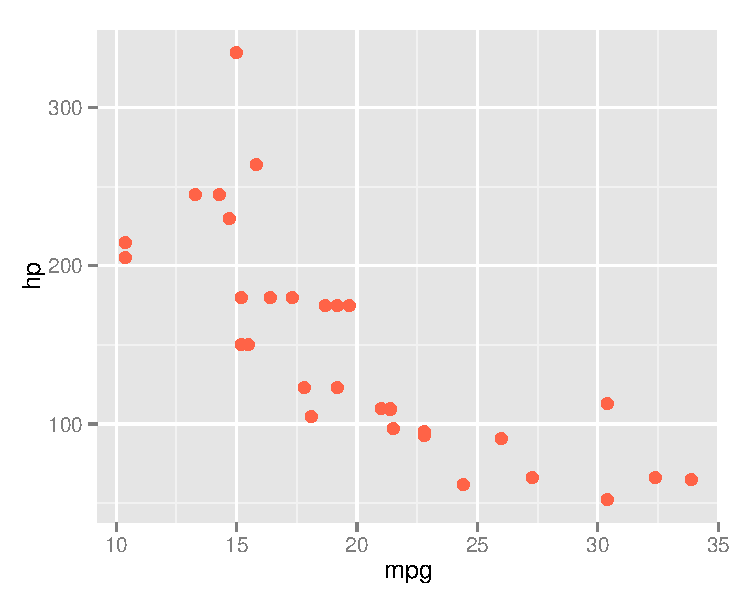
\includegraphics[width=.7\linewidth,height=.6\linewidth]{figure/xyplot_mtcars3-1} 

}



\end{knitrout}
\end{frame}

%------------------------------------------------

\begin{frame}[fragile]
\frametitle{Adding color}
\begin{knitrout}\scriptsize
\definecolor{shadecolor}{rgb}{0.969, 0.969, 0.969}\color{fgcolor}\begin{kframe}
\begin{alltt}
\hlkwd{ggplot}\hlstd{(}\hlkwc{data} \hlstd{= mtcars,} \hlkwd{aes}\hlstd{(}\hlkwc{x} \hlstd{= mpg,} \hlkwc{y} \hlstd{= hp))} \hlopt{+}
  \hlkwd{geom_point}\hlstd{(}\hlkwc{size} \hlstd{=} \hlnum{3}\hlstd{,} \hlkwc{color} \hlstd{=} \hlstr{"#259ff8"}\hlstd{)}
\end{alltt}
\end{kframe}

{\centering 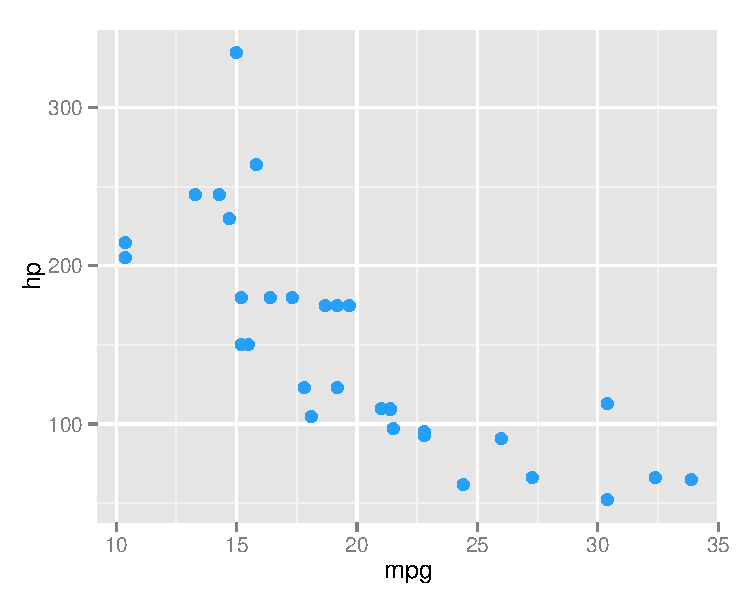
\includegraphics[width=.7\linewidth,height=.6\linewidth]{figure/unnamed-chunk-4-1} 

}



\end{knitrout}
\end{frame}

%------------------------------------------------

\begin{frame}
\frametitle{Test your knowledge}

\bb{Identify the valid hex-color}
\bbi
  \item[A)] \code{"345677"}
  \item[B)] \code{"\#1234567"}
  \item[C)] \code{"\#AAAAAA"}
  \item[D)] \code{"\#GG0033"}
\ei
\eb

\end{frame}

%------------------------------------------------

\begin{frame}[fragile]
\frametitle{Changing points shape}
\begin{knitrout}\scriptsize
\definecolor{shadecolor}{rgb}{0.969, 0.969, 0.969}\color{fgcolor}\begin{kframe}
\begin{alltt}
\hlcom{# 'shape' accepts 'pch' values}
\hlkwd{ggplot}\hlstd{(}\hlkwc{data} \hlstd{= mtcars,} \hlkwd{aes}\hlstd{(}\hlkwc{x} \hlstd{= mpg,} \hlkwc{y} \hlstd{= hp))} \hlopt{+}
  \hlkwd{geom_point}\hlstd{(}\hlkwc{size} \hlstd{=} \hlnum{3}\hlstd{,} \hlkwc{color} \hlstd{=} \hlstr{"tomato"}\hlstd{,} \hlkwc{shape} \hlstd{=} \hlnum{15}\hlstd{)}
\end{alltt}
\end{kframe}

{\centering 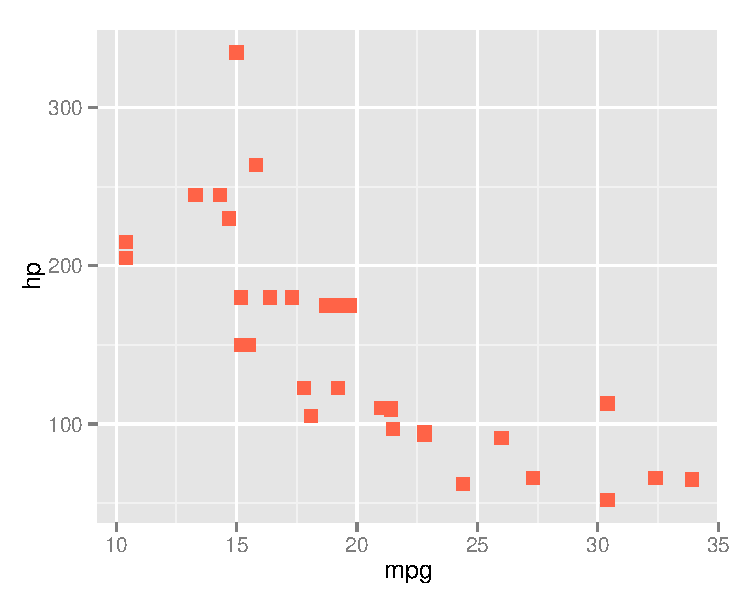
\includegraphics[width=.7\linewidth,height=.6\linewidth]{figure/xyplot_mtcars4-1} 

}



\end{knitrout}
\end{frame}

%------------------------------------------------

\begin{frame}[fragile]
\frametitle{Setting and Mapping}

Aesthetic attributes can be either \textbf{mapped} ---via \code{aes()}--- or \textbf{set}

\begin{knitrout}\footnotesize
\definecolor{shadecolor}{rgb}{0.969, 0.969, 0.969}\color{fgcolor}\begin{kframe}
\begin{alltt}
\hlcom{# mapping aesthetic color}
\hlkwd{ggplot}\hlstd{(mtcars,} \hlkwd{aes}\hlstd{(}\hlkwc{x} \hlstd{= mpg,} \hlkwc{y} \hlstd{= hp))} \hlopt{+}
  \hlkwd{geom_point}\hlstd{(}\hlkwd{aes}\hlstd{(}\hlkwc{color} \hlstd{= cyl))}

\hlcom{# setting aesthetic color}
\hlkwd{ggplot}\hlstd{(mtcars,} \hlkwd{aes}\hlstd{(}\hlkwc{x} \hlstd{= mpg,} \hlkwc{y} \hlstd{= hp))} \hlopt{+}
  \hlkwd{geom_point}\hlstd{(}\hlkwc{color} \hlstd{=} \hlstr{"blue"}\hlstd{)}
\end{alltt}
\end{kframe}
\end{knitrout}

\end{frame}

%------------------------------------------------

\begin{frame}[fragile]
\frametitle{Geom text, and mapping labels}
\begin{knitrout}\scriptsize
\definecolor{shadecolor}{rgb}{0.969, 0.969, 0.969}\color{fgcolor}\begin{kframe}
\begin{alltt}
\hlkwd{ggplot}\hlstd{(}\hlkwc{data} \hlstd{= mtcars,} \hlkwd{aes}\hlstd{(}\hlkwc{x} \hlstd{= mpg,} \hlkwc{y} \hlstd{= hp))} \hlopt{+}
  \hlkwd{geom_text}\hlstd{(}\hlkwd{aes}\hlstd{(}\hlkwc{label} \hlstd{= gear))}
\end{alltt}
\end{kframe}

{\centering 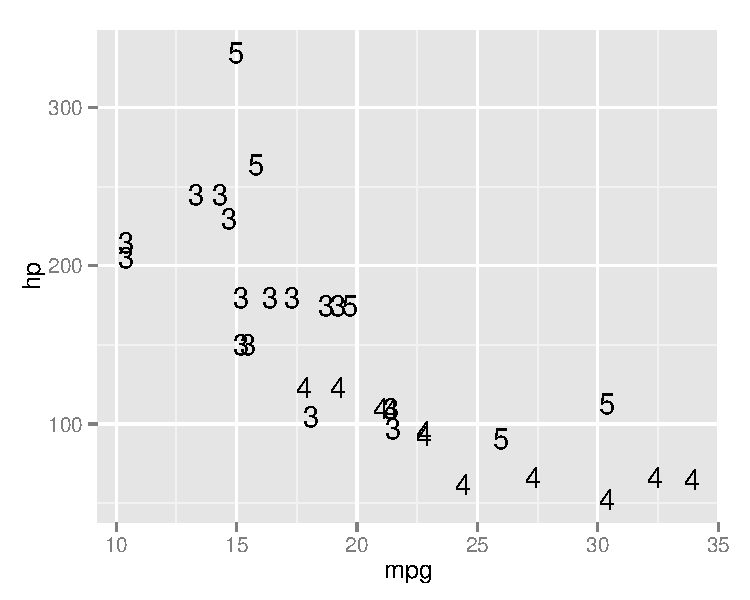
\includegraphics[width=.7\linewidth,height=.6\linewidth]{figure/xyplot_mtcars9-1} 

}



\end{knitrout}

\end{frame}

%------------------------------------------------

\begin{frame}[fragile]
\frametitle{Changing axis labels and title}
\begin{knitrout}\scriptsize
\definecolor{shadecolor}{rgb}{0.969, 0.969, 0.969}\color{fgcolor}\begin{kframe}
\begin{alltt}
\hlkwd{ggplot}\hlstd{(}\hlkwc{data} \hlstd{= mtcars,} \hlkwd{aes}\hlstd{(}\hlkwc{x} \hlstd{= mpg,} \hlkwc{y} \hlstd{= hp))} \hlopt{+}
  \hlkwd{geom_point}\hlstd{(}\hlkwc{size} \hlstd{=} \hlnum{3}\hlstd{,} \hlkwc{color} \hlstd{=} \hlstr{"tomato"}\hlstd{)} \hlopt{+}
  \hlkwd{xlab}\hlstd{(}\hlstr{"miles per gallon"}\hlstd{)} \hlopt{+}
  \hlkwd{ylab}\hlstd{(}\hlstr{"horse power"}\hlstd{)} \hlopt{+}
  \hlkwd{ggtitle}\hlstd{(}\hlstr{"Scatter plot with ggplot2"}\hlstd{)}
\end{alltt}
\end{kframe}

{\centering 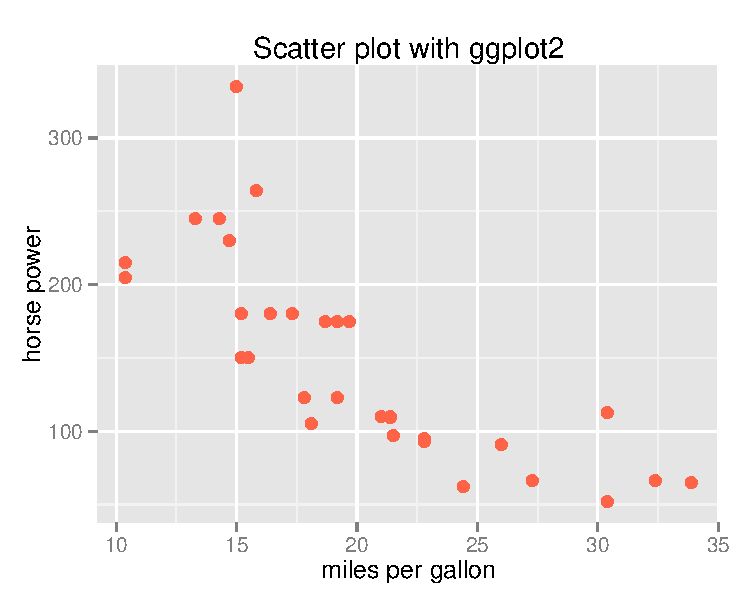
\includegraphics[width=.6\linewidth,height=.5\linewidth]{figure/xyplot_mtcars5-1} 

}



\end{knitrout}
\end{frame}

%------------------------------------------------

\begin{frame}[fragile]
\frametitle{Changing background theme}
\begin{knitrout}\scriptsize
\definecolor{shadecolor}{rgb}{0.969, 0.969, 0.969}\color{fgcolor}\begin{kframe}
\begin{alltt}
\hlkwd{ggplot}\hlstd{(}\hlkwc{data} \hlstd{= mtcars,} \hlkwd{aes}\hlstd{(}\hlkwc{x} \hlstd{= mpg,} \hlkwc{y} \hlstd{= hp))} \hlopt{+}
  \hlkwd{geom_point}\hlstd{(}\hlkwc{size} \hlstd{=} \hlnum{3}\hlstd{,} \hlkwc{color} \hlstd{=} \hlstr{"tomato"}\hlstd{)} \hlopt{+}
  \hlkwd{xlab}\hlstd{(}\hlstr{"miles per gallon"}\hlstd{)} \hlopt{+}
  \hlkwd{ylab}\hlstd{(}\hlstr{"horse power"}\hlstd{)} \hlopt{+}
  \hlkwd{ggtitle}\hlstd{(}\hlstr{"Scatter plot with ggplot2"}\hlstd{)} \hlopt{+}
  \hlkwd{theme_bw}\hlstd{()}
\end{alltt}
\end{kframe}

{\centering 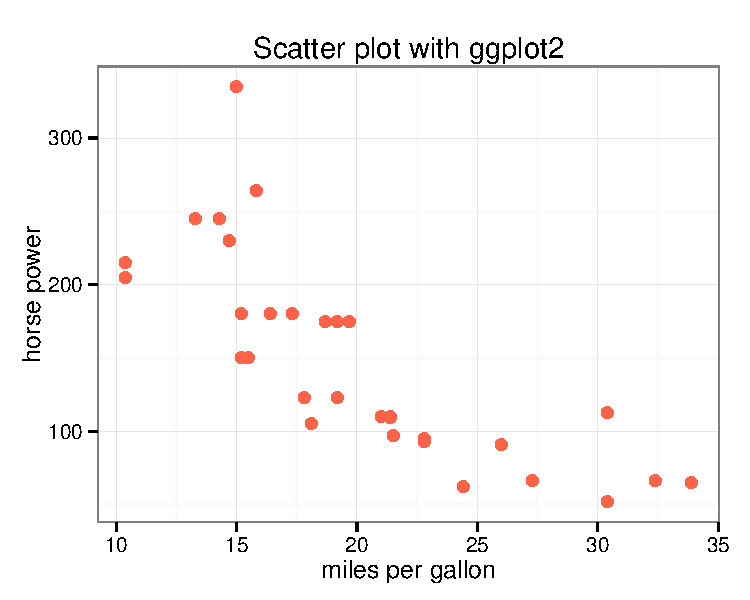
\includegraphics[width=.6\linewidth,height=.5\linewidth]{figure/xyplot_mtcars6-1} 

}



\end{knitrout}
\end{frame}

%------------------------------------------------

\begin{frame}[fragile]
\frametitle{Your turn: Replicate this figure}
\begin{knitrout}\scriptsize
\definecolor{shadecolor}{rgb}{0.969, 0.969, 0.969}\color{fgcolor}

{\centering 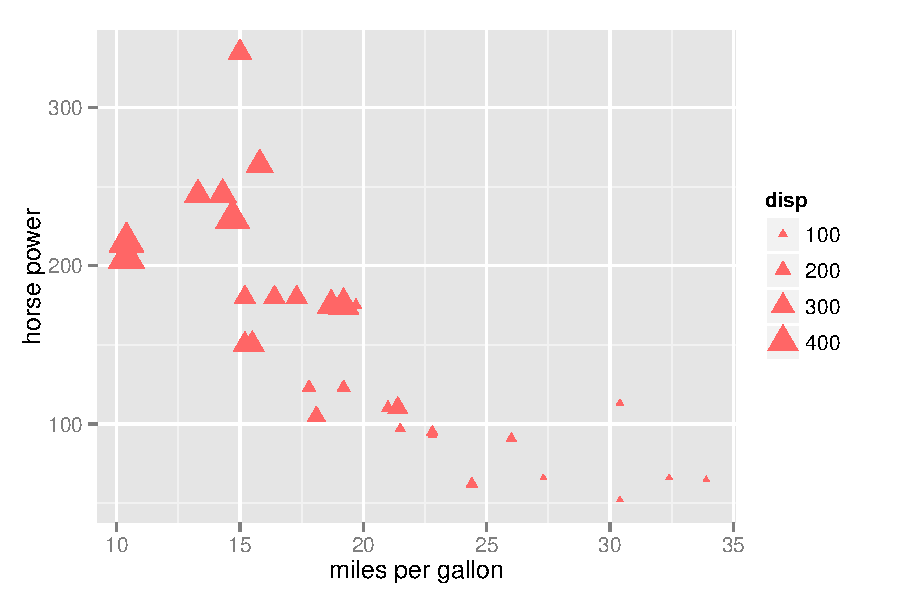
\includegraphics[width=.8\linewidth,height=.6\linewidth]{figure/your_xyplot1-1} 

}



\end{knitrout}
\end{frame}

%------------------------------------------------

\begin{frame}[fragile]
\frametitle{Your turn: Replicate this figure}
\bi
  \item Specify a color in hex notation
  \item Change the shape of the point symbol
  \item Map \code{disp} to attribute size of points
  \item Add axis labels
\ei
\end{frame}

%------------------------------------------------

\begin{frame}[fragile]
\frametitle{Your turn}
\begin{knitrout}\footnotesize
\definecolor{shadecolor}{rgb}{0.969, 0.969, 0.969}\color{fgcolor}\begin{kframe}
\begin{alltt}
\hlkwd{ggplot}\hlstd{(}\hlkwc{data} \hlstd{= mtcars,} \hlkwd{aes}\hlstd{(}\hlkwc{x} \hlstd{= mpg,} \hlkwc{y} \hlstd{= hp))} \hlopt{+}
  \hlkwd{geom_point}\hlstd{(}\hlkwd{aes}\hlstd{(}\hlkwc{size} \hlstd{= disp),}
             \hlkwc{color} \hlstd{=} \hlstr{"#ff6666"}\hlstd{,} \hlkwc{shape} \hlstd{=} \hlnum{17}\hlstd{)} \hlopt{+}
  \hlkwd{xlab}\hlstd{(}\hlstr{"miles per gallon"}\hlstd{)} \hlopt{+}
  \hlkwd{ylab}\hlstd{(}\hlstr{"horse power"}\hlstd{)}
\end{alltt}
\end{kframe}
\end{knitrout}
\end{frame}

%------------------------------------------------

\begin{frame}[fragile]
\frametitle{More geoms}
\begin{knitrout}\scriptsize
\definecolor{shadecolor}{rgb}{0.969, 0.969, 0.969}\color{fgcolor}\begin{kframe}
\begin{alltt}
\hlkwd{ggplot}\hlstd{(}\hlkwc{data} \hlstd{= mtcars,} \hlkwd{aes}\hlstd{(}\hlkwc{x} \hlstd{= mpg,} \hlkwc{y} \hlstd{= hp))} \hlopt{+}
  \hlkwd{geom_point}\hlstd{()} \hlopt{+}
  \hlkwd{geom_smooth}\hlstd{(}\hlkwc{method} \hlstd{=} \hlstr{"lm"}\hlstd{)}
\end{alltt}
\end{kframe}

{\centering 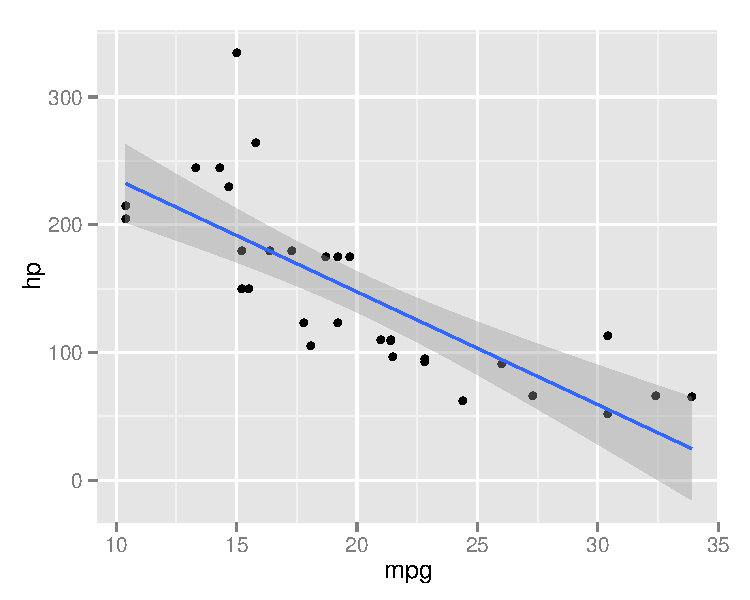
\includegraphics[width=.7\linewidth,height=.6\linewidth]{figure/xyplot_mtcars10-1} 

}



\end{knitrout}

\end{frame}

%------------------------------------------------

\begin{frame}[fragile]
\frametitle{More geoms}
We can map variable to a color aesthetic. Here we map \code{color} to \code{cyl} (cylinders)
\begin{knitrout}\scriptsize
\definecolor{shadecolor}{rgb}{0.969, 0.969, 0.969}\color{fgcolor}\begin{kframe}
\begin{alltt}
\hlkwd{ggplot}\hlstd{(}\hlkwc{data} \hlstd{= mtcars,} \hlkwd{aes}\hlstd{(}\hlkwc{x} \hlstd{= mpg,} \hlkwc{y} \hlstd{= hp))} \hlopt{+}
  \hlkwd{geom_point}\hlstd{(}\hlkwd{aes}\hlstd{(}\hlkwc{color} \hlstd{= cyl))}
\end{alltt}
\end{kframe}

{\centering 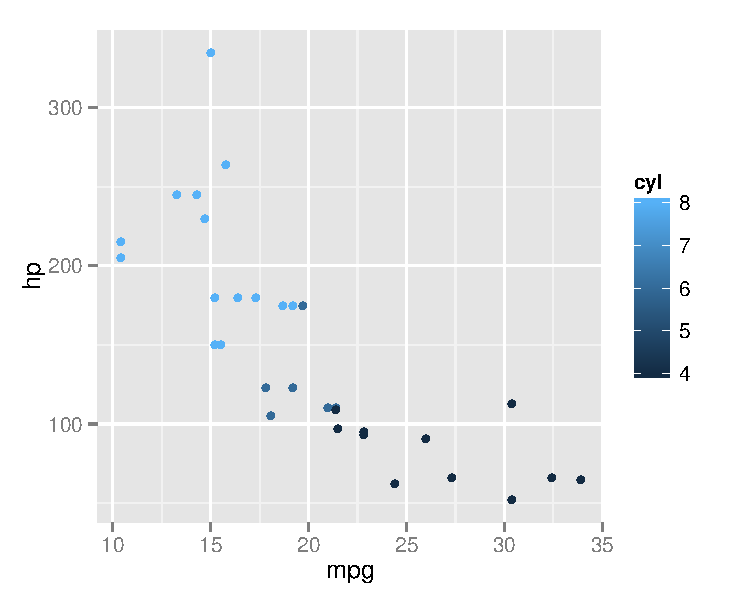
\includegraphics[width=.6\linewidth,height=.5\linewidth]{figure/xyplot_mtcars11-1} 

}



\end{knitrout}

\end{frame}

%------------------------------------------------

\begin{frame}[fragile]
\frametitle{More geoms}
If the variable that maps to color is a factor, then the color scale will change
\begin{knitrout}\scriptsize
\definecolor{shadecolor}{rgb}{0.969, 0.969, 0.969}\color{fgcolor}\begin{kframe}
\begin{alltt}
\hlkwd{ggplot}\hlstd{(}\hlkwc{data} \hlstd{= mtcars,} \hlkwd{aes}\hlstd{(}\hlkwc{x} \hlstd{= mpg,} \hlkwc{y} \hlstd{= hp))} \hlopt{+}
  \hlkwd{geom_point}\hlstd{(}\hlkwd{aes}\hlstd{(}\hlkwc{color} \hlstd{=} \hlkwd{as.factor}\hlstd{(cyl)))}
\end{alltt}
\end{kframe}

{\centering 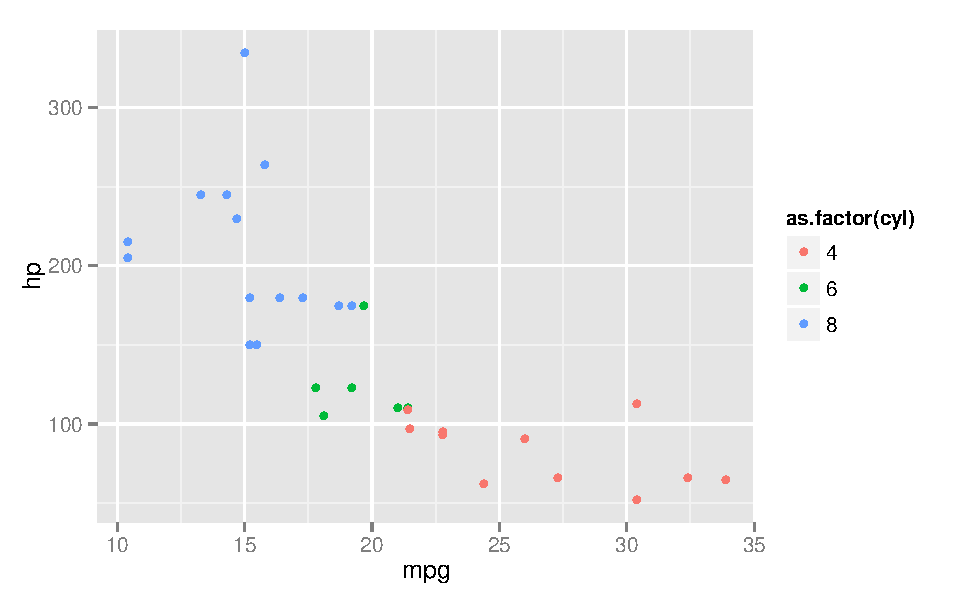
\includegraphics[width=.75\linewidth,height=.5\linewidth]{figure/xyplot_mtcars12-1} 

}



\end{knitrout}

\end{frame}

%------------------------------------------------

\begin{frame}[fragile]
\frametitle{Your turn: Replicate this figure}
\begin{knitrout}\scriptsize
\definecolor{shadecolor}{rgb}{0.969, 0.969, 0.969}\color{fgcolor}

{\centering 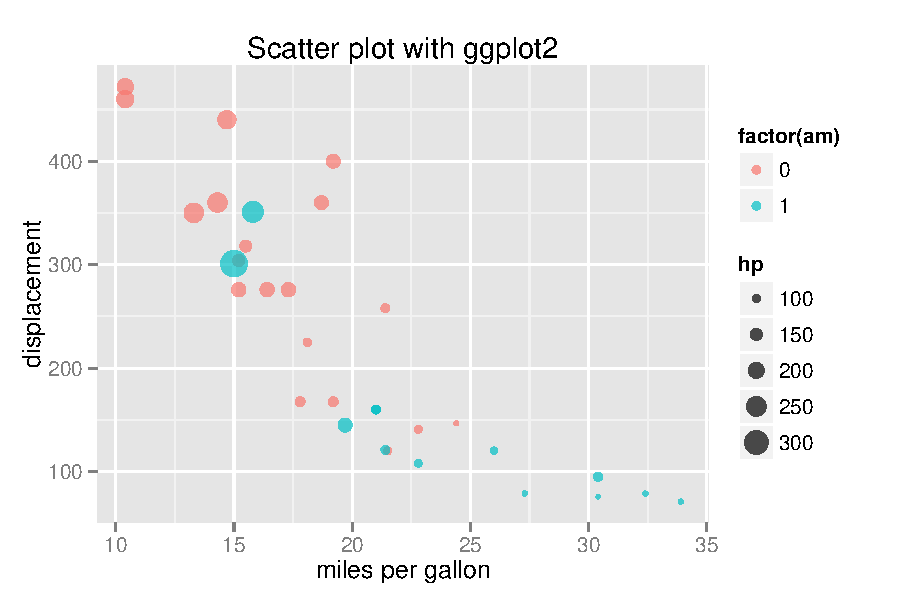
\includegraphics[width=.85\linewidth,height=.6\linewidth]{figure/your_xyplot2-1} 

}



\end{knitrout}
\end{frame}

%------------------------------------------------

\begin{frame}[fragile]
\frametitle{Your turn: example 2}
\bi
  \item Map \code{hp} to attribute size of points
  \item Map \code{am} (as factor) to attribute color points
  \item Add an alpha transparency of 0.7
  \item Change the shape of the point symbol
  \item Add axis labels
  \item Add a title
\ei
\end{frame}

%------------------------------------------------

\begin{frame}[fragile]
\frametitle{Your turn: example 2}
\begin{knitrout}\footnotesize
\definecolor{shadecolor}{rgb}{0.969, 0.969, 0.969}\color{fgcolor}\begin{kframe}
\begin{alltt}
\hlkwd{ggplot}\hlstd{(}\hlkwc{data} \hlstd{= mtcars,} \hlkwd{aes}\hlstd{(}\hlkwc{x} \hlstd{= mpg,} \hlkwc{y} \hlstd{= disp))} \hlopt{+}
  \hlkwd{geom_point}\hlstd{(}\hlkwd{aes}\hlstd{(}\hlkwc{size} \hlstd{= hp,} \hlkwc{color} \hlstd{=} \hlkwd{factor}\hlstd{(am)),}
             \hlkwc{alpha} \hlstd{=} \hlnum{0.7}\hlstd{)} \hlopt{+}
  \hlkwd{xlab}\hlstd{(}\hlstr{"miles per gallon"}\hlstd{)} \hlopt{+}
  \hlkwd{ylab}\hlstd{(}\hlstr{"displacement"}\hlstd{)} \hlopt{+}
  \hlkwd{ggtitle}\hlstd{(}\hlstr{"Scatter plot with ggplot2"}\hlstd{)}
\end{alltt}
\end{kframe}
\end{knitrout}
\end{frame}

%------------------------------------------------

\begin{frame}[fragile]
\frametitle{Histogram}

\begin{knitrout}\scriptsize
\definecolor{shadecolor}{rgb}{0.969, 0.969, 0.969}\color{fgcolor}\begin{kframe}
\begin{alltt}
\hlkwd{ggplot}\hlstd{(}\hlkwc{data} \hlstd{= mtcars,} \hlkwd{aes}\hlstd{(}\hlkwc{x} \hlstd{= mpg))} \hlopt{+}
  \hlkwd{geom_histogram}\hlstd{(}\hlkwc{binwidth} \hlstd{=} \hlnum{2}\hlstd{)}
\end{alltt}
\end{kframe}

{\centering 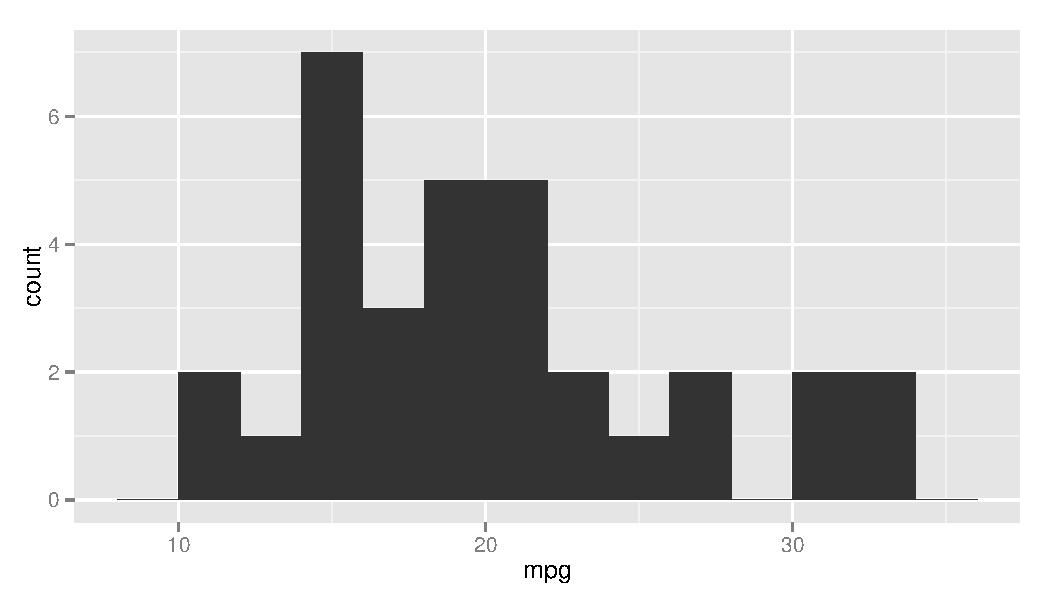
\includegraphics[width=.9\linewidth,height=.5\linewidth]{figure/unnamed-chunk-6-1} 

}



\end{knitrout}

\end{frame}

%------------------------------------------------

\begin{frame}[fragile]
\frametitle{Boxplots}

\begin{knitrout}\scriptsize
\definecolor{shadecolor}{rgb}{0.969, 0.969, 0.969}\color{fgcolor}\begin{kframe}
\begin{alltt}
\hlkwd{ggplot}\hlstd{(}\hlkwc{data} \hlstd{= mtcars,} \hlkwd{aes}\hlstd{(}\hlkwc{x} \hlstd{=} \hlkwd{factor}\hlstd{(cyl),} \hlkwc{y} \hlstd{= mpg))} \hlopt{+}
  \hlkwd{geom_boxplot}\hlstd{()}
\end{alltt}
\end{kframe}

{\centering 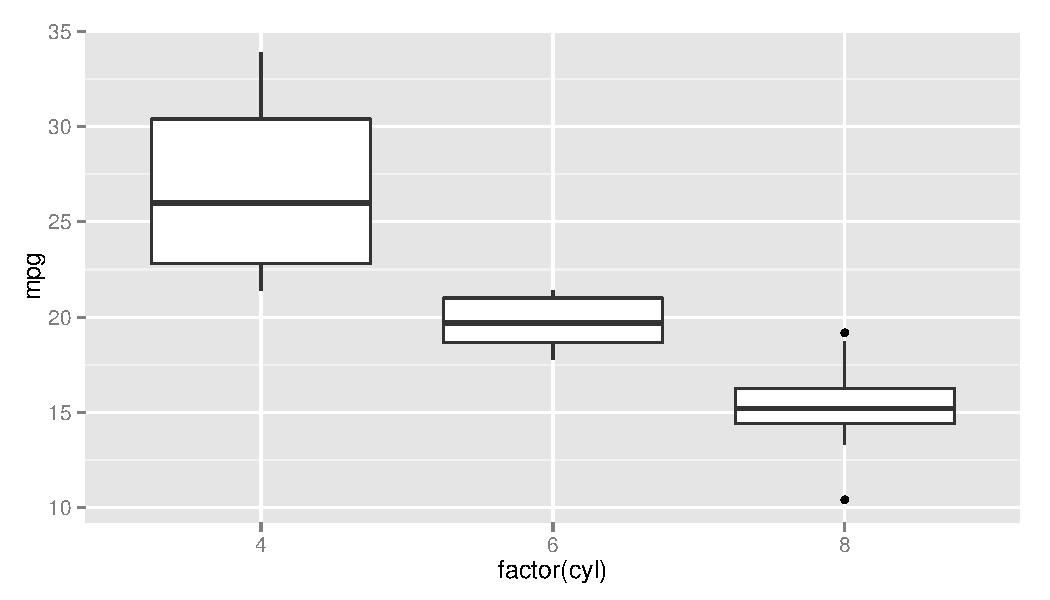
\includegraphics[width=.9\linewidth,height=.5\linewidth]{figure/unnamed-chunk-7-1} 

}



\end{knitrout}

\end{frame}

%------------------------------------------------

\begin{frame}[fragile]
\frametitle{Density Curves}

\begin{knitrout}\scriptsize
\definecolor{shadecolor}{rgb}{0.969, 0.969, 0.969}\color{fgcolor}\begin{kframe}
\begin{alltt}
\hlkwd{ggplot}\hlstd{(}\hlkwc{data} \hlstd{= mtcars,} \hlkwd{aes}\hlstd{(}\hlkwc{x} \hlstd{= mpg))} \hlopt{+}
  \hlkwd{geom_density}\hlstd{()}
\end{alltt}
\end{kframe}

{\centering 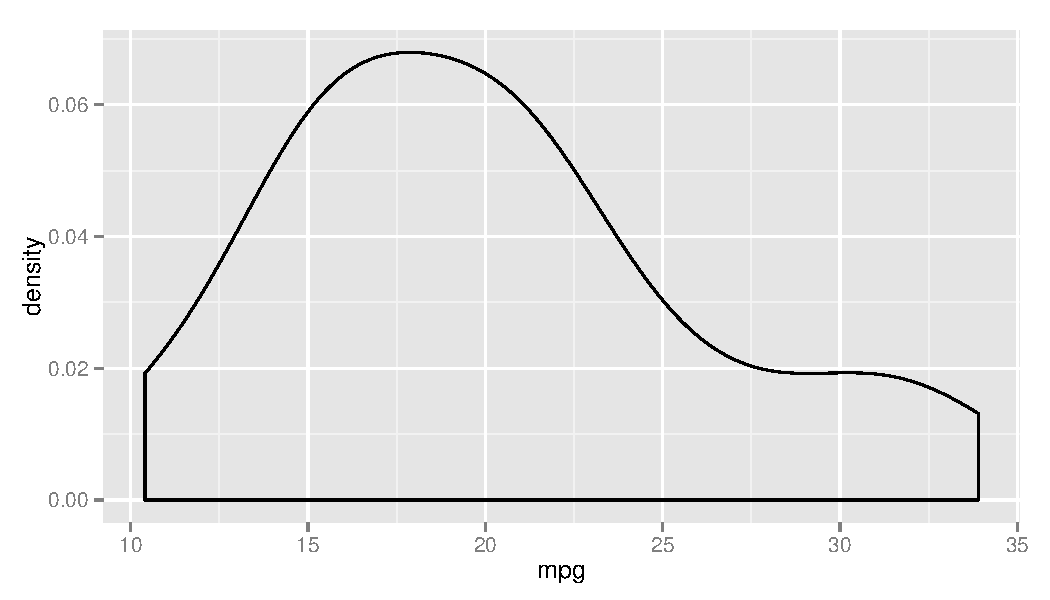
\includegraphics[width=.9\linewidth,height=.5\linewidth]{figure/unnamed-chunk-8-1} 

}



\end{knitrout}

\end{frame}

%------------------------------------------------

\begin{frame}[fragile]
\frametitle{Density Curves}

\begin{knitrout}\scriptsize
\definecolor{shadecolor}{rgb}{0.969, 0.969, 0.969}\color{fgcolor}\begin{kframe}
\begin{alltt}
\hlkwd{ggplot}\hlstd{(}\hlkwc{data} \hlstd{= mtcars,} \hlkwd{aes}\hlstd{(}\hlkwc{x} \hlstd{= mpg))} \hlopt{+}
  \hlkwd{geom_density}\hlstd{(}\hlkwc{fill} \hlstd{=} \hlstr{"#c6b7f5"}\hlstd{)}
\end{alltt}
\end{kframe}

{\centering 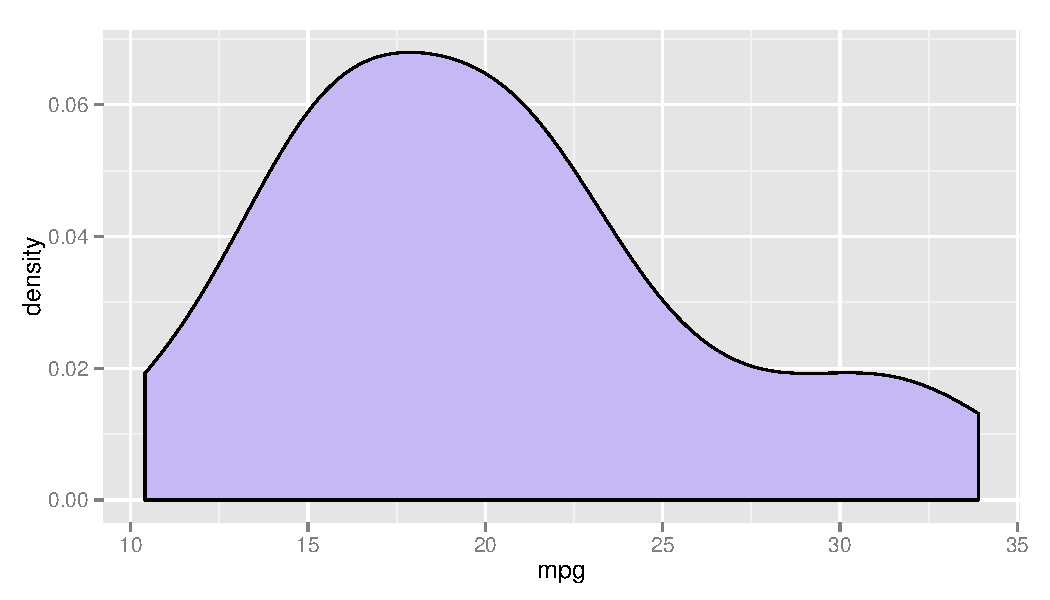
\includegraphics[width=.9\linewidth,height=.5\linewidth]{figure/unnamed-chunk-9-1} 

}



\end{knitrout}

\end{frame}

%------------------------------------------------

\begin{frame}[fragile]
\frametitle{Density Curves}

\begin{knitrout}\scriptsize
\definecolor{shadecolor}{rgb}{0.969, 0.969, 0.969}\color{fgcolor}\begin{kframe}
\begin{alltt}
\hlkwd{ggplot}\hlstd{(}\hlkwc{data} \hlstd{= mtcars,} \hlkwd{aes}\hlstd{(}\hlkwc{x} \hlstd{= mpg))} \hlopt{+}
  \hlkwd{geom_density}\hlstd{(}\hlkwc{fill} \hlstd{=} \hlstr{"#c6b7f5"}\hlstd{,} \hlkwc{alpha} \hlstd{=} \hlnum{0.4}\hlstd{)}
\end{alltt}
\end{kframe}

{\centering 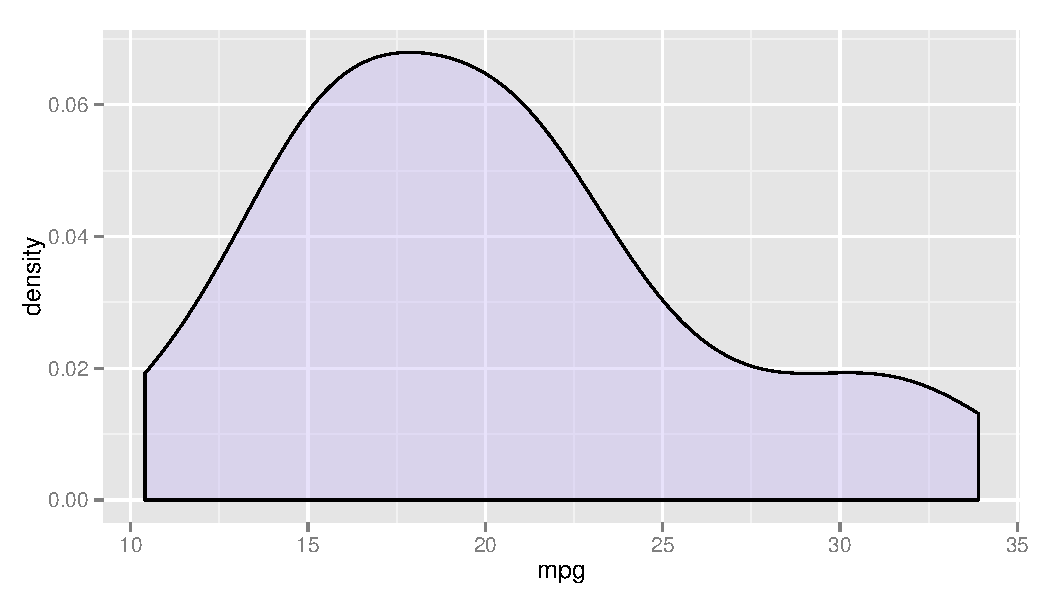
\includegraphics[width=.9\linewidth,height=.5\linewidth]{figure/unnamed-chunk-10-1} 

}



\end{knitrout}

\end{frame}

%------------------------------------------------

\begin{frame}[fragile]
\frametitle{Density Curves}

\begin{knitrout}\scriptsize
\definecolor{shadecolor}{rgb}{0.969, 0.969, 0.969}\color{fgcolor}\begin{kframe}
\begin{alltt}
\hlkwd{ggplot}\hlstd{(}\hlkwc{data} \hlstd{= mtcars,} \hlkwd{aes}\hlstd{(}\hlkwc{x} \hlstd{= mpg))} \hlopt{+}
  \hlkwd{geom_line}\hlstd{(}\hlkwc{stat} \hlstd{=} \hlstr{'density'}\hlstd{,} \hlkwc{col} \hlstd{=} \hlstr{"#a868c0"}\hlstd{,} \hlkwc{size} \hlstd{=} \hlnum{2}\hlstd{)}
\end{alltt}
\end{kframe}

{\centering 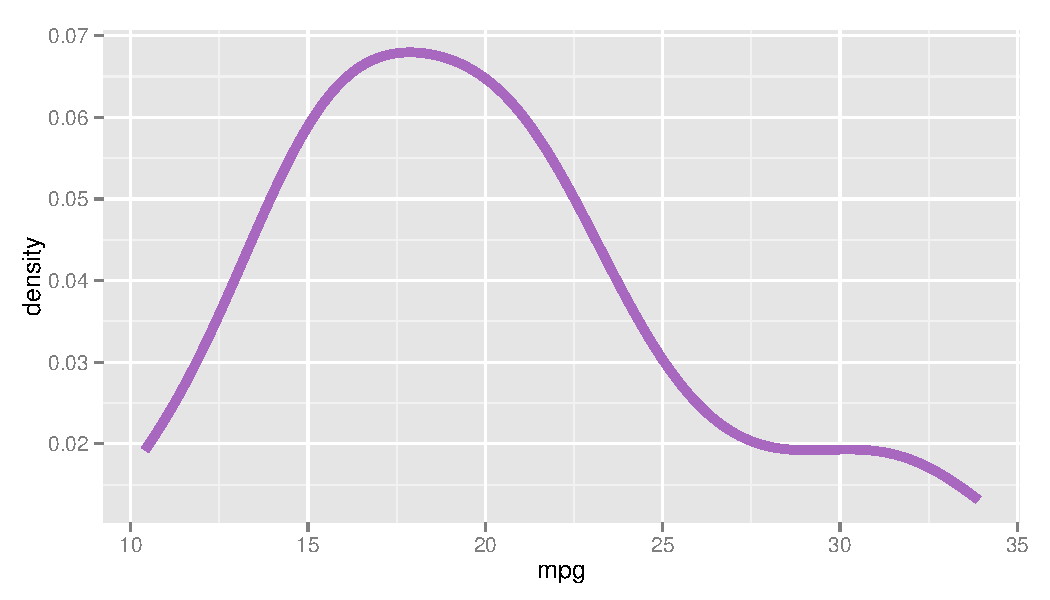
\includegraphics[width=.9\linewidth,height=.5\linewidth]{figure/unnamed-chunk-11-1} 

}



\end{knitrout}

\end{frame}

%------------------------------------------------

\begin{frame}[fragile]
\frametitle{Density Curves}

\begin{knitrout}\scriptsize
\definecolor{shadecolor}{rgb}{0.969, 0.969, 0.969}\color{fgcolor}\begin{kframe}
\begin{alltt}
\hlkwd{ggplot}\hlstd{(}\hlkwc{data} \hlstd{= mtcars,} \hlkwd{aes}\hlstd{(}\hlkwc{x} \hlstd{= mpg))} \hlopt{+}
  \hlkwd{geom_density}\hlstd{(}\hlkwc{fill} \hlstd{=} \hlstr{'#a868c0'}\hlstd{)} \hlopt{+}
  \hlkwd{geom_line}\hlstd{(}\hlkwc{stat} \hlstd{=} \hlstr{'density'}\hlstd{,} \hlkwc{col} \hlstd{=} \hlstr{"#a868c0"}\hlstd{,} \hlkwc{size} \hlstd{=} \hlnum{2}\hlstd{)}
\end{alltt}
\end{kframe}

{\centering 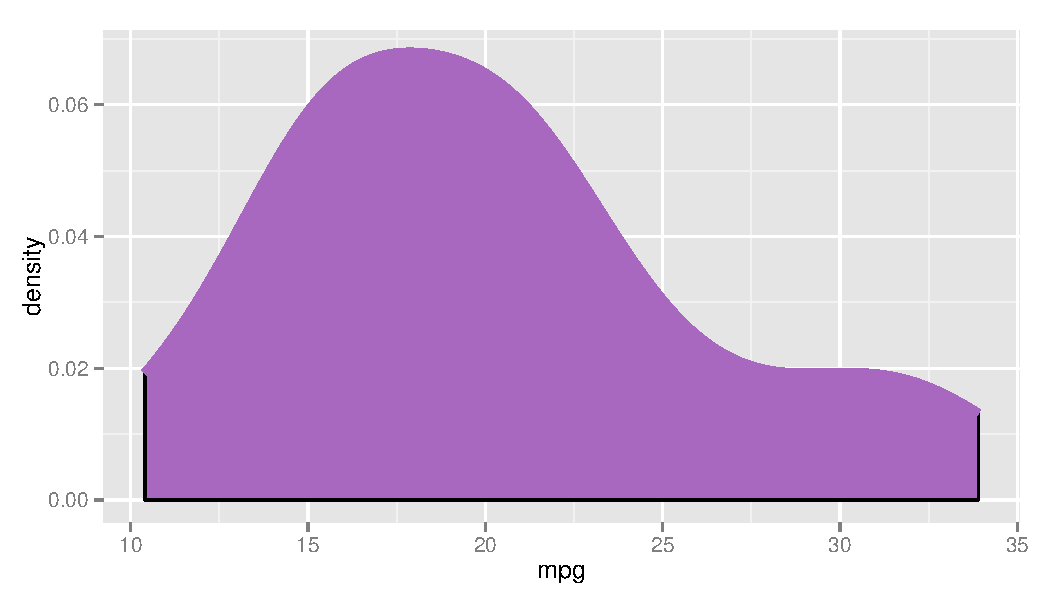
\includegraphics[width=.9\linewidth,height=.5\linewidth]{figure/unnamed-chunk-12-1} 

}



\end{knitrout}

\end{frame}

%------------------------------------------------

\begin{frame}
\begin{center}
\Huge{\hilit{\code{ggplot} objects}}
\end{center}
\end{frame}

%------------------------------------------------

\begin{frame}[fragile]
\frametitle{Plot objects}
You can assign a plot to a new object (this won't plot anything):
\begin{knitrout}\footnotesize
\definecolor{shadecolor}{rgb}{0.969, 0.969, 0.969}\color{fgcolor}\begin{kframe}
\begin{alltt}
\hlstd{mpg_hp} \hlkwb{<-} \hlkwd{ggplot}\hlstd{(}\hlkwc{data} \hlstd{= mtcars,} \hlkwd{aes}\hlstd{(}\hlkwc{x} \hlstd{= mpg,} \hlkwc{y} \hlstd{= hp))} \hlopt{+}
  \hlkwd{geom_point}\hlstd{(}\hlkwc{size} \hlstd{=} \hlnum{3}\hlstd{,} \hlkwc{color} \hlstd{=} \hlstr{"tomato"}\hlstd{)}
\end{alltt}
\end{kframe}
\end{knitrout}

To show the actual plot associated to the object \code{mpg\_hp} use the function \code{print()}
\begin{knitrout}\footnotesize
\definecolor{shadecolor}{rgb}{0.969, 0.969, 0.969}\color{fgcolor}\begin{kframe}
\begin{alltt}
\hlkwd{print}\hlstd{(mpg_hp)}
\end{alltt}
\end{kframe}
\end{knitrout}
\end{frame}

%------------------------------------------------

\begin{frame}[fragile]
\frametitle{\code{"ggplot2"} objects}

\bb{working with ggplot objects, we can ...}
\bi
  \item define a basic plot, to which we can add or change layers without typing everything again
  \item render it on screen with \code{print()}
  \item describe its structure with \code{summary()}
  \item render it to disk with \code{ggsave()}
  \item save a cached copy to disk with \code{save()}
\ei
\eb

\end{frame}

%------------------------------------------------

\begin{frame}[fragile]
\frametitle{}
Adding a title and axis labels to a ggplot2 object:
\begin{knitrout}\scriptsize
\definecolor{shadecolor}{rgb}{0.969, 0.969, 0.969}\color{fgcolor}\begin{kframe}
\begin{alltt}
\hlstd{mpg_hp} \hlopt{+} \hlkwd{ggtitle}\hlstd{(}\hlstr{"Scatter plot with ggplot2"}\hlstd{)} \hlopt{+}
  \hlkwd{xlab}\hlstd{(}\hlstr{"miles per gallon"}\hlstd{)} \hlopt{+} \hlkwd{ylab}\hlstd{(}\hlstr{"horse power"}\hlstd{)}
\end{alltt}
\end{kframe}

{\centering 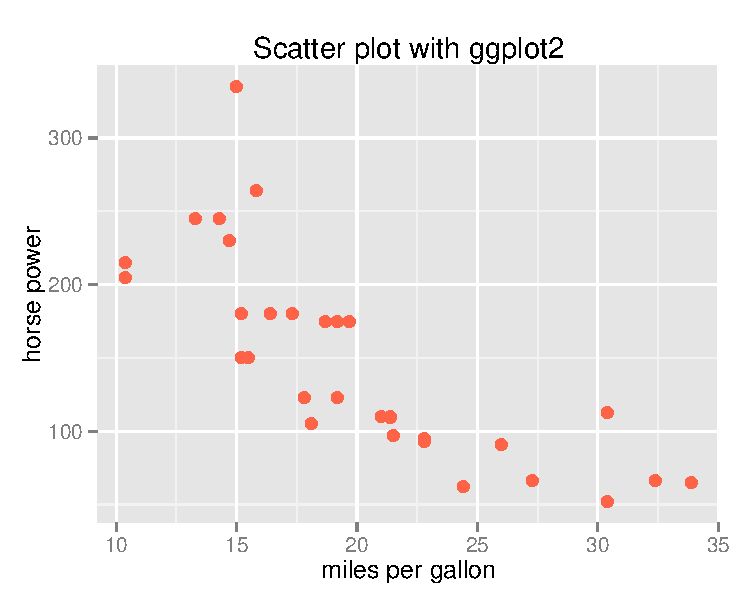
\includegraphics[width=.6\linewidth,height=.5\linewidth]{figure/xyplot_mtcars8-1} 

}



\end{knitrout}

\end{frame}

%------------------------------------------------

\begin{frame}[fragile]
\frametitle{Your turn: example 3}
Create the following ggplot object:
\begin{knitrout}\footnotesize
\definecolor{shadecolor}{rgb}{0.969, 0.969, 0.969}\color{fgcolor}\begin{kframe}
\begin{alltt}
\hlcom{# ggplot object}
\hlstd{obj} \hlkwb{<-} \hlkwd{ggplot}\hlstd{(}\hlkwc{data} \hlstd{= mtcars,}
         \hlkwd{aes}\hlstd{(}\hlkwc{x} \hlstd{= mpg,} \hlkwc{y} \hlstd{= hp,} \hlkwc{label} \hlstd{=} \hlkwd{rownames}\hlstd{(mtcars)))}
\end{alltt}
\end{kframe}
\end{knitrout}

Add more layers to the object \code"{"obj"} in order to replicate the figure in the following slide:
\end{frame}

%------------------------------------------------

\begin{frame}[fragile]
\frametitle{Your turn: example 3}
\begin{knitrout}\scriptsize
\definecolor{shadecolor}{rgb}{0.969, 0.969, 0.969}\color{fgcolor}

{\centering 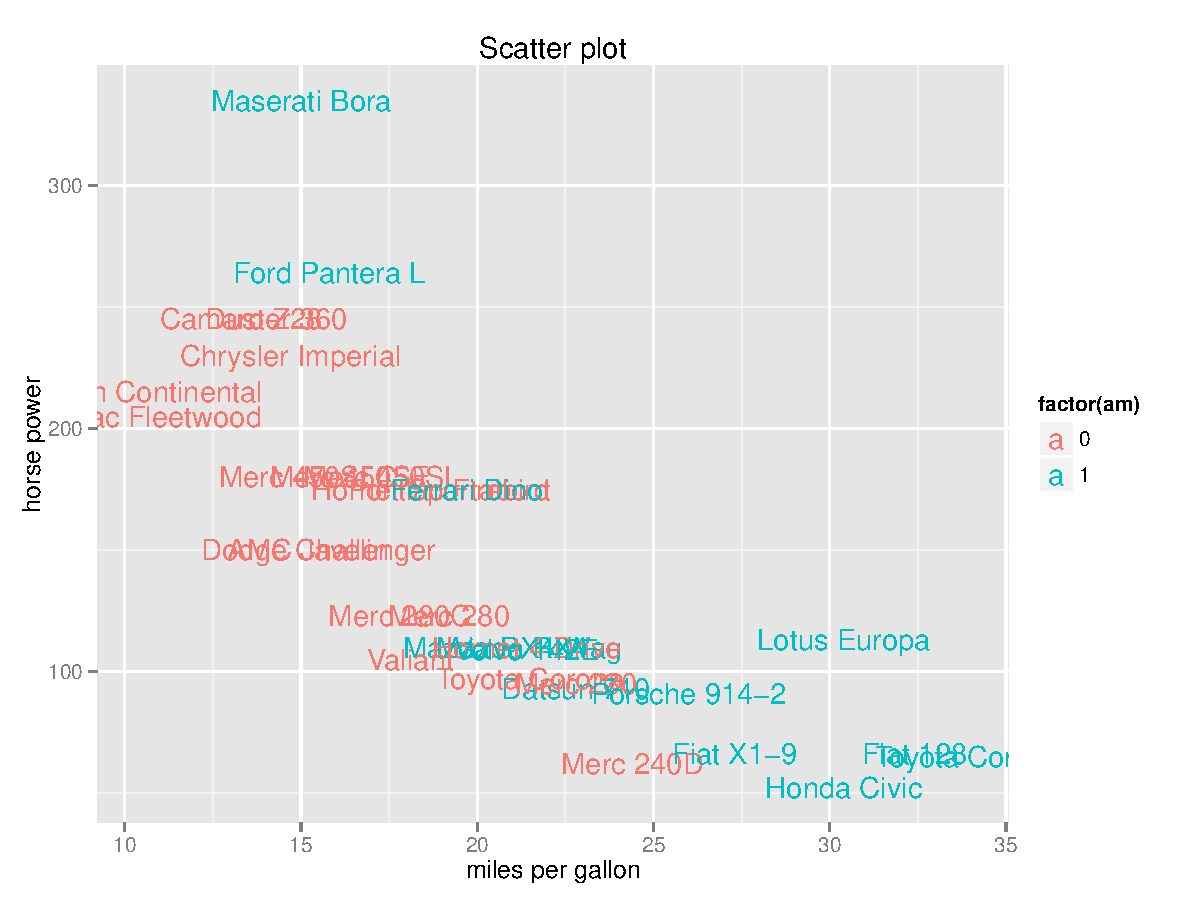
\includegraphics[width=.8\linewidth,height=.6\linewidth]{figure/your_xyplot3-1} 

}



\end{knitrout}
\end{frame}

%------------------------------------------------

\begin{frame}[fragile]
\frametitle{Your turn: example 3}
\begin{knitrout}\footnotesize
\definecolor{shadecolor}{rgb}{0.969, 0.969, 0.969}\color{fgcolor}\begin{kframe}
\begin{alltt}
\hlstd{obj} \hlopt{+}
  \hlkwd{geom_text}\hlstd{(}\hlkwd{aes}\hlstd{(}\hlkwc{color} \hlstd{=} \hlkwd{factor}\hlstd{(am)))} \hlopt{+}
  \hlkwd{ggtitle}\hlstd{(}\hlstr{"Scatter plot"}\hlstd{)} \hlopt{+}
  \hlkwd{xlab}\hlstd{(}\hlstr{"miles per gallon"}\hlstd{)} \hlopt{+}
  \hlkwd{ylab}\hlstd{(}\hlstr{"horse power"}\hlstd{)}
\end{alltt}
\end{kframe}
\end{knitrout}
\end{frame}

%------------------------------------------------

\begin{frame}
\begin{center}
\Huge{\hilit{Scales}}
\end{center}
\end{frame}

%------------------------------------------------

\begin{frame}
\frametitle{Scales}

\bi
  \item The \textbf{scales} component encompases the ideas of both axes and legends on plots, e.g.:
  \item Axes can be continuous or discrete
  \item Legends involve colors, symbol shapes, size, etc
  \bi
    \item \code{scale\_x\_continuous}
    \item \code{scale\_y\_continuous}
    \item \code{scale\_color\_manual}
  \ei
  \item \textbf{scales} will often automatically generate appropriate scales for plots
  \item Explicitly adding a scale component overrides the default scale
\ei

\end{frame}

%------------------------------------------------

\begin{frame}[fragile]
\frametitle{Continuous axis scales}
Use \code{scale\_x\_continuous()} to modify the default values in the $x$ axis
\begin{knitrout}\footnotesize
\definecolor{shadecolor}{rgb}{0.969, 0.969, 0.969}\color{fgcolor}\begin{kframe}
\begin{alltt}
\hlkwd{ggplot}\hlstd{(}\hlkwc{data} \hlstd{= mtcars,} \hlkwd{aes}\hlstd{(}\hlkwc{x} \hlstd{= mpg,} \hlkwc{y} \hlstd{= hp))} \hlopt{+}
  \hlkwd{geom_point}\hlstd{(}\hlkwd{aes}\hlstd{(}\hlkwc{color} \hlstd{=} \hlkwd{factor}\hlstd{(am)))} \hlopt{+}
  \hlkwd{scale_x_continuous}\hlstd{(}\hlkwc{name} \hlstd{=} \hlstr{"miles per gallon"}\hlstd{,}
                     \hlkwc{limits} \hlstd{=} \hlkwd{c}\hlstd{(}\hlnum{10}\hlstd{,} \hlnum{40}\hlstd{),}
                     \hlkwc{breaks} \hlstd{=} \hlkwd{c}\hlstd{(}\hlnum{10}\hlstd{,} \hlnum{20}\hlstd{,} \hlnum{30}\hlstd{,} \hlnum{40}\hlstd{))}
\end{alltt}
\end{kframe}
\end{knitrout}
\end{frame}

%------------------------------------------------

\begin{frame}[fragile]
\frametitle{Continuous axis scales}
\begin{knitrout}\footnotesize
\definecolor{shadecolor}{rgb}{0.969, 0.969, 0.969}\color{fgcolor}

{\centering 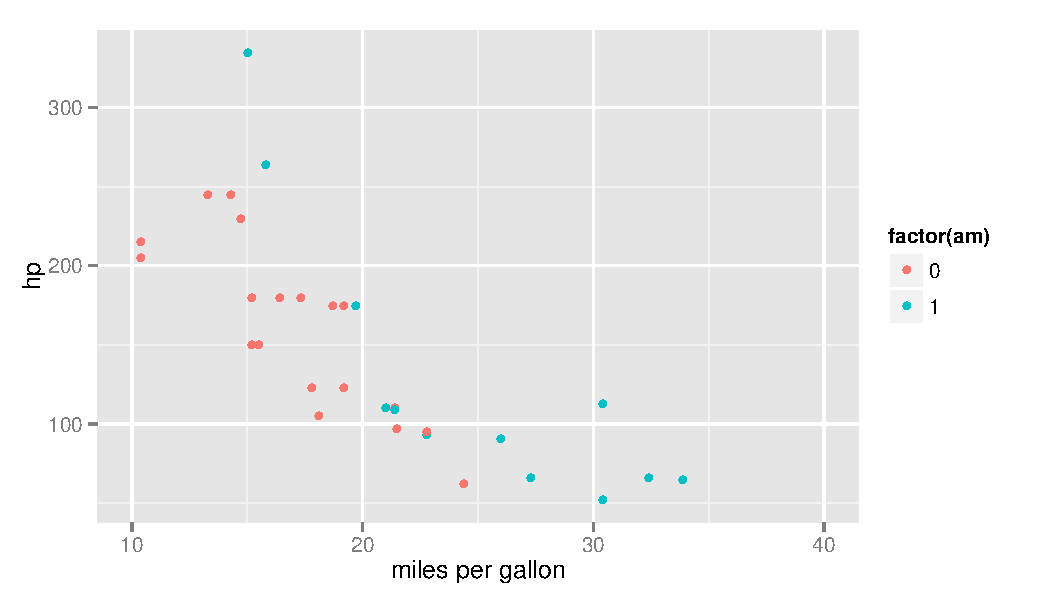
\includegraphics[width=.9\linewidth,height=.5\linewidth]{figure/scale_x-1} 

}



\end{knitrout}
\end{frame}

%------------------------------------------------

\begin{frame}[fragile]
\frametitle{Continuous axis scales}
Use \code{scale\_y\_continuous()} to modify the default values in the $y$ axis
\begin{knitrout}\footnotesize
\definecolor{shadecolor}{rgb}{0.969, 0.969, 0.969}\color{fgcolor}\begin{kframe}
\begin{alltt}
\hlkwd{ggplot}\hlstd{(}\hlkwc{data} \hlstd{= mtcars,} \hlkwd{aes}\hlstd{(}\hlkwc{x} \hlstd{= mpg,} \hlkwc{y} \hlstd{= hp))} \hlopt{+}
  \hlkwd{geom_point}\hlstd{(}\hlkwd{aes}\hlstd{(}\hlkwc{color} \hlstd{=} \hlkwd{factor}\hlstd{(am)))} \hlopt{+}
  \hlkwd{scale_x_continuous}\hlstd{(}\hlkwc{name} \hlstd{=} \hlstr{"miles per gallon"}\hlstd{,}
                     \hlkwc{limits} \hlstd{=} \hlkwd{c}\hlstd{(}\hlnum{10}\hlstd{,} \hlnum{40}\hlstd{),}
                     \hlkwc{breaks} \hlstd{=} \hlkwd{c}\hlstd{(}\hlnum{10}\hlstd{,} \hlnum{20}\hlstd{,} \hlnum{30}\hlstd{,} \hlnum{40}\hlstd{))} \hlopt{+}
  \hlkwd{scale_y_continuous}\hlstd{(}\hlkwc{name} \hlstd{=} \hlstr{"horsepower"}\hlstd{,}
                     \hlkwc{limits} \hlstd{=} \hlkwd{c}\hlstd{(}\hlnum{50}\hlstd{,} \hlnum{350}\hlstd{),}
                     \hlkwc{breaks} \hlstd{=} \hlkwd{seq}\hlstd{(}\hlnum{50}\hlstd{,} \hlnum{350}\hlstd{,} \hlkwc{by} \hlstd{=} \hlnum{50}\hlstd{))}
\end{alltt}
\end{kframe}
\end{knitrout}
\end{frame}

%------------------------------------------------

\begin{frame}[fragile]
\frametitle{Continuous axis scales}
\begin{knitrout}\footnotesize
\definecolor{shadecolor}{rgb}{0.969, 0.969, 0.969}\color{fgcolor}

{\centering 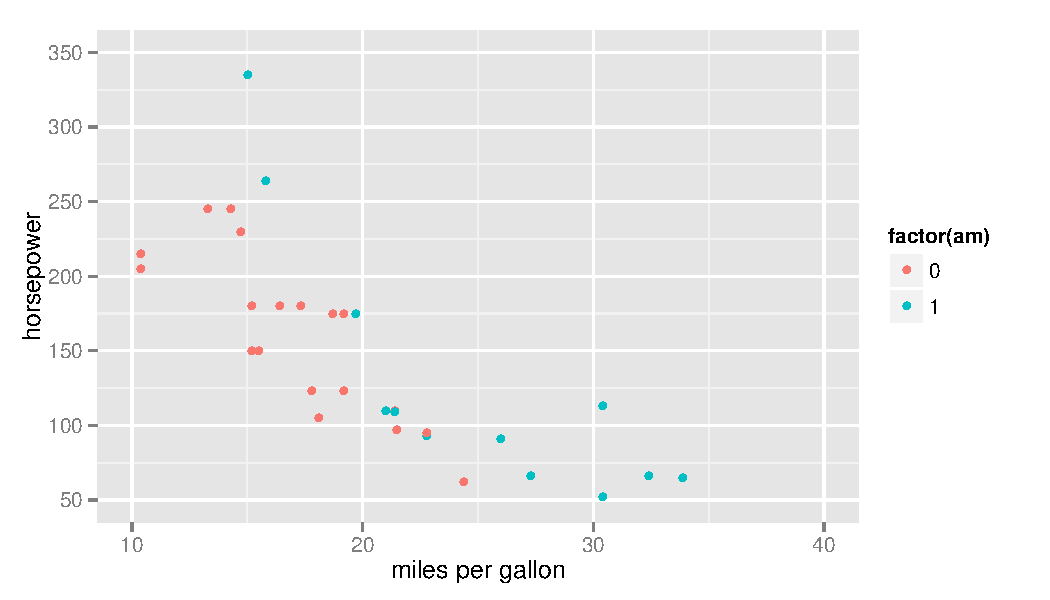
\includegraphics[width=.9\linewidth,height=.5\linewidth]{figure/scale_y-1} 

}



\end{knitrout}
\end{frame}

%------------------------------------------------

\begin{frame}[fragile]
\frametitle{Example: color scale}

Use \code{scale\_color\_manual()} to modify the colors associated to a factor
\begin{knitrout}\footnotesize
\definecolor{shadecolor}{rgb}{0.969, 0.969, 0.969}\color{fgcolor}\begin{kframe}
\begin{alltt}
\hlkwd{ggplot}\hlstd{(}\hlkwc{data} \hlstd{= mtcars,} \hlkwd{aes}\hlstd{(}\hlkwc{x} \hlstd{= mpg,} \hlkwc{y} \hlstd{= hp))} \hlopt{+}
  \hlkwd{geom_point}\hlstd{(}\hlkwd{aes}\hlstd{(}\hlkwc{color} \hlstd{=} \hlkwd{factor}\hlstd{(am)))} \hlopt{+}
  \hlkwd{scale_color_manual}\hlstd{(}\hlkwc{values} \hlstd{=} \hlkwd{c}\hlstd{(}\hlstr{"orange"}\hlstd{,} \hlstr{"purple"}\hlstd{))}
\end{alltt}
\end{kframe}
\end{knitrout}

\end{frame}

%------------------------------------------------

\begin{frame}[fragile]
\frametitle{Example: color scale}

\begin{knitrout}\footnotesize
\definecolor{shadecolor}{rgb}{0.969, 0.969, 0.969}\color{fgcolor}

{\centering 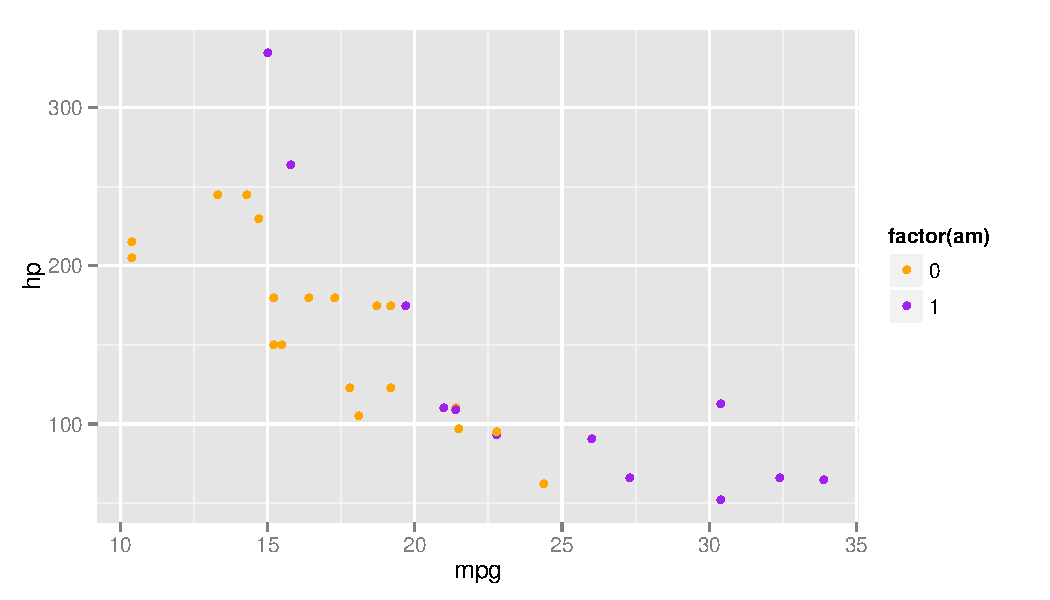
\includegraphics[width=.9\linewidth,height=.5\linewidth]{figure/color_manual-1} 

}



\end{knitrout}

\end{frame}

%------------------------------------------------

\begin{frame}[fragile]
\frametitle{Example: modifying legend}

Modifying legends depends on the type of scales (e.g. color, shapes, size, etc)
\begin{knitrout}\footnotesize
\definecolor{shadecolor}{rgb}{0.969, 0.969, 0.969}\color{fgcolor}\begin{kframe}
\begin{alltt}
\hlkwd{ggplot}\hlstd{(}\hlkwc{data} \hlstd{= mtcars,} \hlkwd{aes}\hlstd{(}\hlkwc{x} \hlstd{= mpg,} \hlkwc{y} \hlstd{= hp))} \hlopt{+}
  \hlkwd{geom_point}\hlstd{(}\hlkwd{aes}\hlstd{(}\hlkwc{color} \hlstd{=} \hlkwd{factor}\hlstd{(am)))} \hlopt{+}
  \hlkwd{scale_color_manual}\hlstd{(}\hlkwc{values} \hlstd{=} \hlkwd{c}\hlstd{(}\hlstr{"orange"}\hlstd{,} \hlstr{"purple"}\hlstd{),}
                     \hlkwc{name} \hlstd{=} \hlstr{"transmission"}\hlstd{,}
                     \hlkwc{labels} \hlstd{=} \hlkwd{c}\hlstd{(}\hlstr{'no'}\hlstd{,} \hlstr{'yes'}\hlstd{))}
\end{alltt}
\end{kframe}
\end{knitrout}
\end{frame}

%------------------------------------------------

\begin{frame}[fragile]
\frametitle{Example: modifying legend}

\begin{knitrout}\footnotesize
\definecolor{shadecolor}{rgb}{0.969, 0.969, 0.969}\color{fgcolor}

{\centering 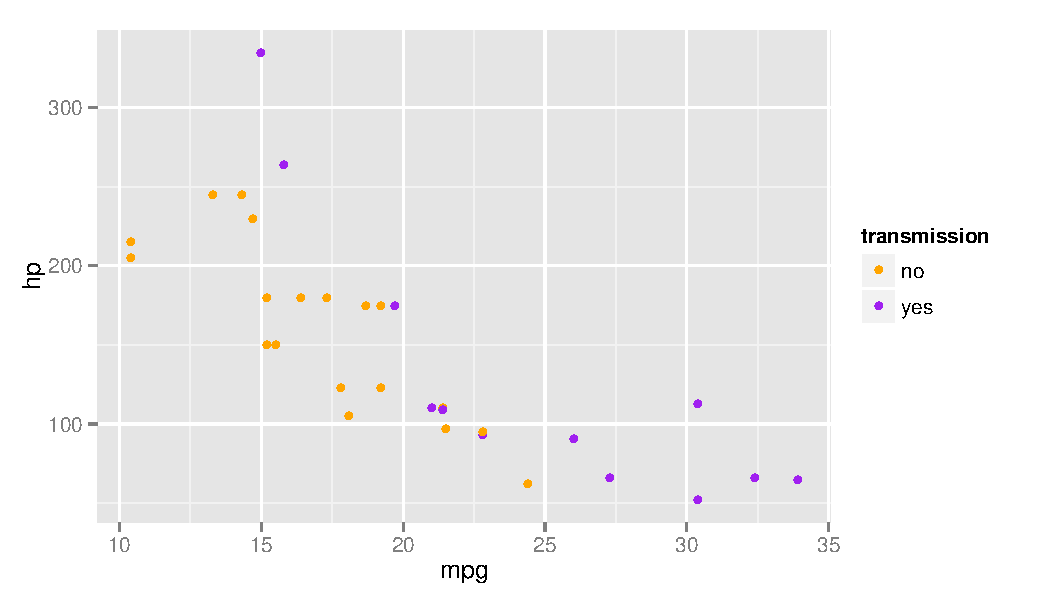
\includegraphics[width=.9\linewidth,height=.5\linewidth]{figure/legend_guide-1} 

}



\end{knitrout}
\end{frame}

%------------------------------------------------

\begin{frame}
\begin{center}
\Huge{\hilit{Faceting}}
\end{center}
\end{frame}

%------------------------------------------------

\begin{frame}[fragile]
\frametitle{Faceting with \code{facet\_wrap()}}

\begin{knitrout}\scriptsize
\definecolor{shadecolor}{rgb}{0.969, 0.969, 0.969}\color{fgcolor}\begin{kframe}
\begin{alltt}
\hlkwd{ggplot}\hlstd{(}\hlkwc{data} \hlstd{= mtcars,} \hlkwd{aes}\hlstd{(}\hlkwc{x} \hlstd{= mpg,} \hlkwc{y} \hlstd{= hp))} \hlopt{+}
  \hlkwd{geom_point}\hlstd{(}\hlkwc{color} \hlstd{=} \hlstr{"#3088f0"}\hlstd{)} \hlopt{+}
  \hlkwd{facet_wrap}\hlstd{(}\hlopt{~} \hlstd{cyl)}
\end{alltt}
\end{kframe}

{\centering 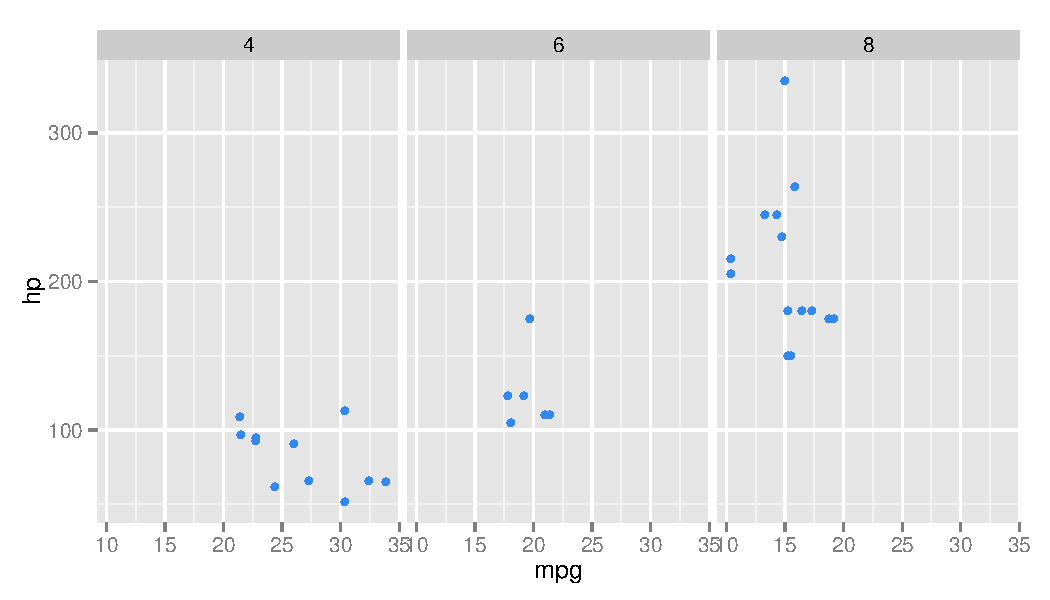
\includegraphics[width=.9\linewidth,height=.5\linewidth]{figure/unnamed-chunk-15-1} 

}



\end{knitrout}

\end{frame}

%------------------------------------------------

\begin{frame}[fragile]
\frametitle{Faceting with \code{facet\_grid()}}

\begin{knitrout}\scriptsize
\definecolor{shadecolor}{rgb}{0.969, 0.969, 0.969}\color{fgcolor}\begin{kframe}
\begin{alltt}
\hlkwd{ggplot}\hlstd{(}\hlkwc{data} \hlstd{= mtcars,} \hlkwd{aes}\hlstd{(}\hlkwc{x} \hlstd{= mpg,} \hlkwc{y} \hlstd{= hp))} \hlopt{+}
  \hlkwd{geom_point}\hlstd{(}\hlkwc{color} \hlstd{=} \hlstr{"#3088f0"}\hlstd{)} \hlopt{+}
  \hlkwd{facet_grid}\hlstd{(cyl} \hlopt{~} \hlstd{.)}
\end{alltt}
\end{kframe}

{\centering 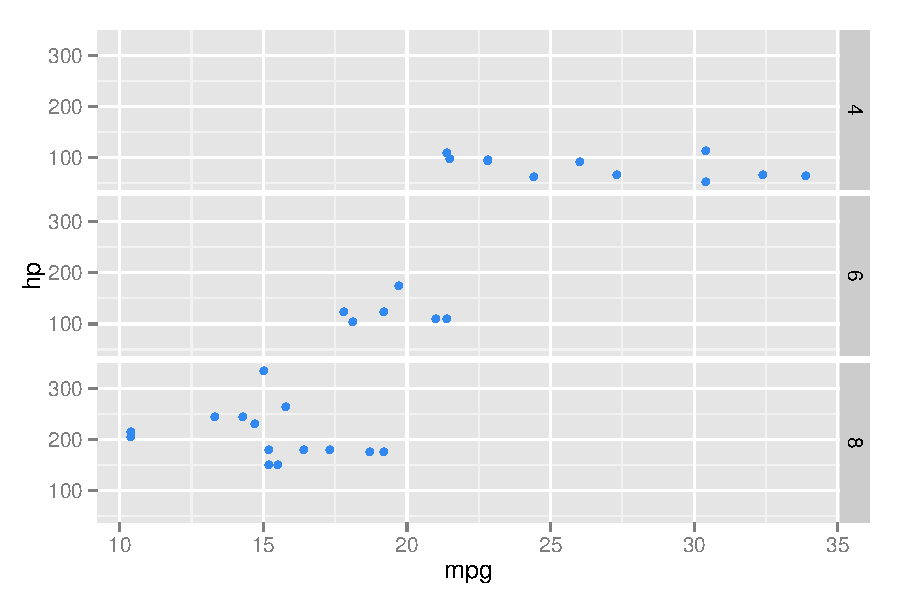
\includegraphics[width=.8\linewidth,height=.5\linewidth]{figure/unnamed-chunk-16-1} 

}



\end{knitrout}

\end{frame}

%------------------------------------------------

\begin{frame}[fragile]
\frametitle{Faceting with \code{facet\_grid()}}

\begin{knitrout}\scriptsize
\definecolor{shadecolor}{rgb}{0.969, 0.969, 0.969}\color{fgcolor}\begin{kframe}
\begin{alltt}
\hlkwd{ggplot}\hlstd{(}\hlkwc{data} \hlstd{= mtcars,} \hlkwd{aes}\hlstd{(}\hlkwc{x} \hlstd{= mpg,} \hlkwc{y} \hlstd{= hp))} \hlopt{+}
  \hlkwd{geom_point}\hlstd{(}\hlkwc{color} \hlstd{=} \hlstr{"#3088f0"}\hlstd{)} \hlopt{+}
  \hlkwd{facet_grid}\hlstd{(.} \hlopt{~} \hlstd{cyl)}
\end{alltt}
\end{kframe}

{\centering 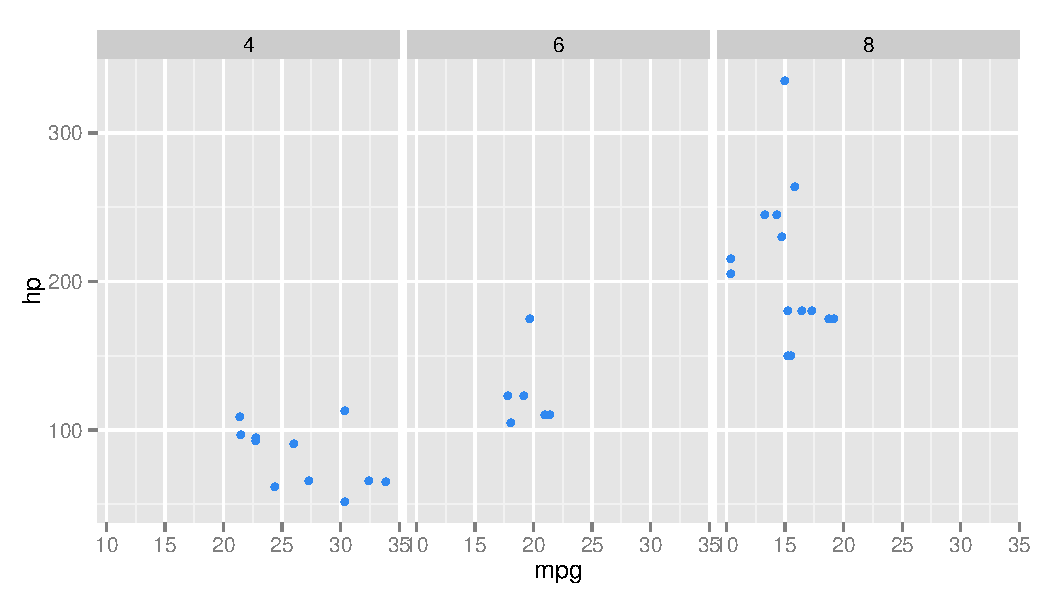
\includegraphics[width=.9\linewidth,height=.5\linewidth]{figure/unnamed-chunk-17-1} 

}



\end{knitrout}

\end{frame}

%------------------------------------------------

\begin{frame}
\frametitle{Layered Grammar}

About \code{"ggplot2"}
\bi
  \item Key concept: \textbf{layer} (layered grammar of graphics)
  \item Designed to work in a layered fashion
  \item Starting with a layer showing the data
  \item Then adding layers of annotations and statistical transformations
  \item Core idea: independents components combined togehter
\ei

\end{frame}

%------------------------------------------------

\begin{frame}
\frametitle{Some Concepts}

\bi
  \item the \textbf{data} to be visualized
  \item a set of \textbf{aesthetic mappings} describing how varibales are mapped to aesthetic attributes
  \item geometric objects, \textbf{geoms}, representing what you  see on the plot (points, lines, etc)
  \item statistical transformations, \textbf{stats}, summarizing data in various ways
  \item \textbf{scales} that map values in the data space to values in an aesthetic space
  \item a coordinate system, \textbf{coord}, describing how data coordinates are mapped to the plane of the graphic
  \item a \textbf{faceting} specification describing how to break up the data into subsets and to displays those subsets
\ei

\end{frame}

%------------------------------------------------

\end{document}
